\documentclass[11pt]{report}
\usepackage[backend=bibtex,style=numeric]{biblatex}
\usepackage[utf8]{inputenc}
\usepackage[english]{babel}
\usepackage[margin=1in]{geometry}
\usepackage{csquotes}
\usepackage{titlesec}
\usepackage[acronym]{glossaries}
\usepackage{mathtools}

\newcommand{\dd}[1]{\mathrm{d}#1}

\bibliography{references}

\title{\textbf{Improving Image Analysis Techniques}}
\author{
\begin{tabular}[t]{cc}
Champion Théophile \\
University of Kent \\
tmac2@kent.ac.uk \\
\end{tabular}
}
\date{\today}

\makeglossaries

\newglossaryentry{task_learning}
{
    name=Task learning,
    description={Task or supervised learning refer to the algorithms that aims to solve a task. In task learning, the expected output is known and part of the expected mapping is given to the models during the learning}
}
\newglossaryentry{model_learning}
{
    name=Model learning,
    description={Model or unsupersised learning refer to the algorithms that aims to create a model of the data. In model learning, the expected output is unknown and the models search for correlations, clusters or structures in the data}
}
 
\newacronym{cnn}{CNN}{Convolutional Neural Network}
\newacronym{conv_net}{ConvNet}{Convolutional Neural Network}
\newacronym{cpca}{CPCA}{Conditional Principal Component Analysis}
\newacronym{kwta}{kWTA}{k-Winners-Take-All}
\newacronym{hcnn}{HCNN}{Hebbian Convolutional Neural Network}
\newacronym{cpu}{CPU}{Central Processing Unit}
\newacronym{gpu}{GPU}{Graphics Processing Unit}

\begin{document}

\maketitle

\tableofcontents

\glsaddall
\printglossary[type=\acronymtype, nonumberlist]
\printglossary[type=main, nonumberlist]

\newpage

\chapter{Introduction}

Image analysis is the field that aims to extract meaning from images. This is an important area of research in machine learning, which has found application from the reading of bar coded tags to the detection of cancerous tumors. It is needless to say that any improvement of the state-of-the-art will have an impact on a lot of domains. This thesis proprose new ideas to improve the convolutional neural network, which is the most popular model in the field.

\section{Objectives}

%TODO

\section{Overview of Contents}

\paragraph{Chapter \ref{related_work}:} Present image analysis techiques as well as notions relevant to the chapter \ref{model_and_task_learning}.
\paragraph{Chapter \ref{model_and_task_learning}:} Propose a new model that learn from the structure of the data.
\paragraph{Chapter \ref{model_implementation}:} Dive into the implementation details of the model.
\paragraph{Chapter \ref{result_and_analysis}:} Analyse the model in terms of accuracy, learning speed and features learned.
\paragraph{Chapter \ref{conclusion}:} Conclude the paper and propose future research directions.

\chapter{Realted Work} \label{related_work}

\section{Convolutional Neural Network}

The \acrshort{cnn} or \acrshort{conv_net} architecture \cite{NIPS1989_293} is a deep neural network learning by backpropagation. It is composed of two kind of nodes: convoltion and pooling. The convolution node contains kernels that will be slide through the image with step size defined by the strides. In recent implementation \cite{5537907} non-linear activation is added after the weighted sum produce by the kernels such as:
\begin{equation}
y_{convolution} = \sigma(z)\ \ \ with\ \ \ z = \sum_{i} x_i \times w_i
\end{equation}
where $y$ is the kernel's output for a specific position in the image, $i$ iterate through all the input as show by the indexes in figure \ref{fig:conv_net}, $x$ are the inputs, $w$ are the kernel's weights and $\sigma$ is the non-linear activation function. Also, the use of local normalization allows local competition between the kernels. The pooling node allow to reduce the dimensionality and making the model invariant to small local variation of its inputs. In the original version \textcite{NIPS1989_293} the pooling applied local average, i.e. mean pooling. More recently, the max pooling have shown better results \cite{10.1007/978-3-642-15825-4_10} by taking the highest value from the pooling kernel such as:
\begin{equation}
y_{mean}\ =\ \frac{1}{|x|}\ \times\ \sum_{i} x_i\ \ \ and\ \ \ y_{max}\ =\ \max_{i}\ x_i
\end{equation}
where $y_{mean}$ and $y_{max}$ are the output of the mean and max pooling for a specific position in the image, $i$ iterate through all the inputs of the pooling kernel, $x$ are the inputs of the pooling kernel, $|x|$ is the number of inputs in the pooling kernel and $w$ are the kernel's weights. Finally, \textcite{DBLP:journals/corr/abs-1811-12231} recently show that CNNs are bias towards texture and describe a method based on image style transfer \cite{Gatys_2016_CVPR}, which increase the shape bias as well as the accuracy.

\begin{figure}[h]
\centering
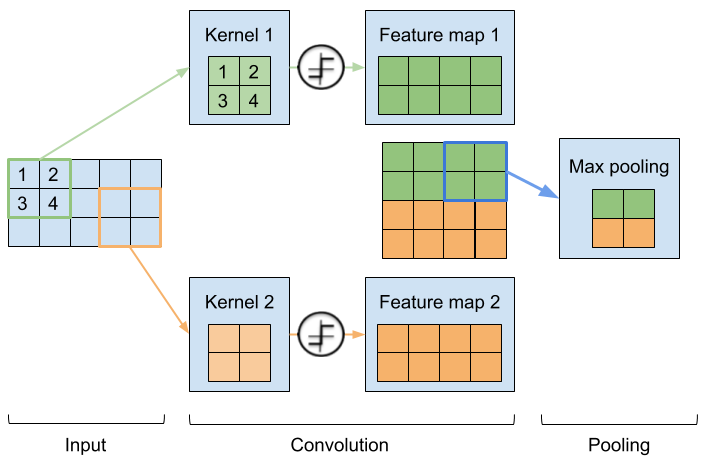
\includegraphics[width=12cm, height=7cm]{conv_net}
\caption{This figure illustrates the convoltion and pooling nodes of the \acrshort{conv_net}. In this example there is two kernels of size 2x2 with stride 1x1, which produce two feature maps. Each element in the feature maps are produced by taking the weighted sum of the kernel's input and passing the result through a non-linear activation function. Then the 2x2 max pooling is applied to each feature map to produce the final output.}
\label{fig:conv_net}
\end{figure}
\section{Deep \acrshort{conv_net}}

This section aims to motivate the improvement of the \acrshort{conv_net} by giving an overview of the varity of model based on it and the multitude of application domains.

\paragraph{Object detection:} Object detection is the field dedictated to the recognition of objects inside images. Over the recent years many models have been proposed to pull the error on the ImageNet data set \cite{imagenet_cvpr09} down. It started with the VGGNet \cite{DBLP:journals/corr/RussakovskyDSKSMHKKBBF14} and the AlexNet \cite{DBLP:journals/cacm/KrizhevskySH17}, which are simply deeper \acrshort{cnn}s. Then the GoogleNet \cite{DBLP:conf/cvpr/SzegedyLJSRAEVR15} introduced the Inception Module, which is able to extract multi-level features from the same input. Indeed, the Inception Module is using kernels of various size, i.e. 1x1, 3x3 and 5x5, to extract features from its inputs. Finally, the ResNet architechture \cite{DBLP:conf/cvpr/HeZRS16} introduced the idea of skip connections where some connections are directly linked to other nodes much higer in the hierachy. The lastest archieved a top-5 error rate of 3.57\% on the ImageNet data set, which is composed of 1000 classes of objects.\newline

\noindent All those models shared the same building blocks (i.e. convolution and pooling nodes) and have been successfully applied to the extraction of text from images, face recognition and scence understanding for autonomous vehicles.

\paragraph{Image segmentation:} Image segmentation is another important task in computer vision, which constists of a pixelwise binary prediction. The model is trained to predict one for all pixels that belongs to a class and zero otherwise. The state-of-the-art in image segmentation are architechture like UNet \cite{DBLP:conf/miccai/RonnebergerFB15} and LinkNet \cite{DBLP:conf/vcip/ChaurasiaC17}. Those architecture are composed of two parts, i.e. an encoder and a decoder. The encoder tranform the input image into a more compact representation that can then be unfold by the decoder to produce the final output.\newline

\noindent Needless to say that image segmentation models can be used to precisely determined the boundary of an object. Another advantage of this technique is that it can be used in collaboration with classical object detection to improve the accuracy of both the segmentation and the classification \cite{DBLP:conf/cvpr/KendallGC18}. The idea is that the encoder remains the same but several tasks are learned from it. The image segement task used the encoder as before while the object detection model used the features that it produce to to performs object detection.

\section{Conditional Principal Component Analysis}

The following explanation are based on the chapter 4 of \textcite{OReilly:2000:CEC:557205:chap4}. Hebbian learning is a biologically plausible and unsupervised learning thechnique based on the idea that neurons that trigger together must strentened their connection. The simplest learning rule in hevbbian learning as follow:

\begin{equation}
\Delta w_{ij} = \epsilon y_jx_i\ \ \ with\ \ \ y_j = \sum_{i}{x_i \times w_{ij}}
\end{equation}

\noindent where $\epsilon$ is the learning rate, $x_i$ is the i-th input, $y_j$ is the j-th output neuron, $w_{ij}$ is the i-th weight of the j-th neuron and $\Delta w_{ij}$ is the update for the weight $w_{ij}$. It can be show that this learning rule learned the first principal component of the data, but this technque has many limitations. First, the weights will become infinitly large as the neurons learn. This can be fix by using the Oja's rule, which normalize the weights update:

\begin{equation}
\Delta w_{ij} = \epsilon (x_iy_j - y_j^2w_{ij})
\end{equation}

\noindent Second, if many neurons are trained using the Oja's rule they will all learn the same component. This can be fix by using the Sanger's rule, which substract the information already explained by the first components:

\begin{equation}
\Delta w_{ij} = \epsilon (x_{stranger}y_j - y_j^2w_{ij})\ \ \ with\ \ \ x_{stranger} = x_i - \sum_{k = 1}^{j - 1}{y_kw_{ik}}
\end{equation}

\noindent Finally, all of the previous learning rules compute the principal component over all the data points. This become a problem when the data is very heterogeneous. Indeed, in the case of the figure \ref{fig:heterogeneous_data} (a) the component learned by such methods will correspond to the blue line, which does not represent well the shape of the data. In this case it is preferable to focus on only one of the two clusters as shows in figure \ref{fig:heterogeneous_data} (b) where the bottom-most cluster is ignored. This is the idea behind \acrshort{cpca}, indeed, in \acrshort{cpca} the neuron will relies on a conditioning function and learn only for learn for a subset of the data. The conditioning function used in this paper will be explained in the next section. The learning rule in \acrshort{cpca} is defined as follow:

\begin{equation}
\Delta w_{ij} = \epsilon y_j (x_i - w_{ij})
\end{equation}

\noindent This learning rule force each weigth $w_{ij}$ to tends to represent the probability of $x_i$ given that the neuron trigger, i.e. $w_{ij} = P(x_i = 1 | y_j = 1)$.

\begin{figure}[h]
\centering
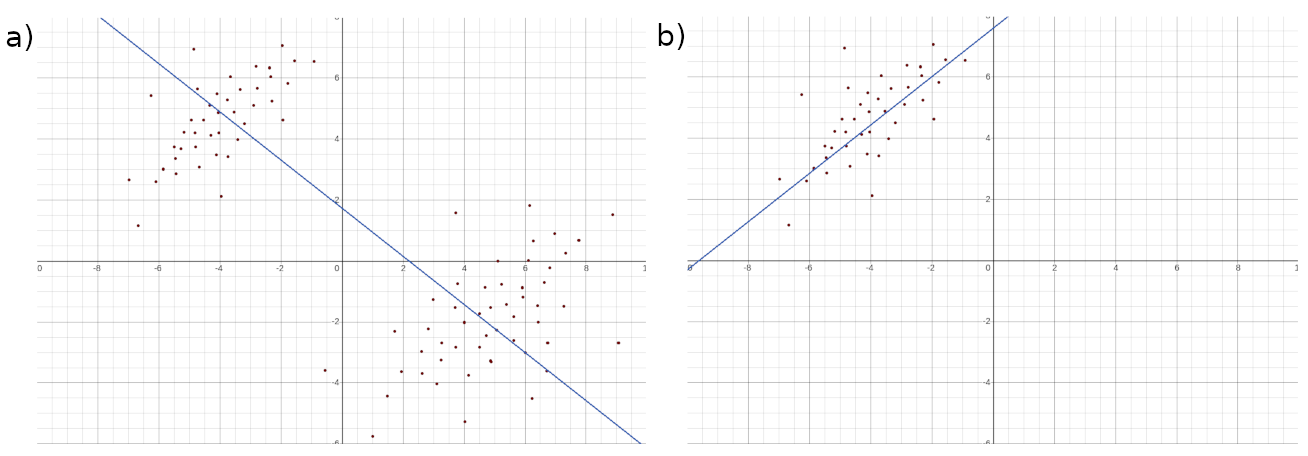
\includegraphics[width=15cm, height=5cm]{heterogeneous_data}
\caption{This figure shows heterogenous data points belonging to two clusters. On the right the first principal component is computed over all the data points. On the left the bottom-most cluster is ignored and the first principal component is computed only over the data points of the top-most cluster.}
\label{fig:heterogeneous_data}
\end{figure}

\section{K-Winner-Take-All} \label{sec:kwta}

The need for a conditioning function in \acrshort{cpca} have been highlighted in the previous section. This section presents the k-Winner-Take-All method that enable such conditioning. The k-Winner-Take-All aims to make only a subset of $k$ neurons to be active for each input. This can be archieved by either inhibiting all the neurons until only $k$ of them remaind active or by forcing the activation to $n - k$ neurons to zero, where $n$ is the total number of neuron in the node.\newline

Independently of the method chosen only the $k$ neurons which have the highest activation will remaind active. Those neurons are the ones whose weights fitted the best the input pattern. Since, the learning rule in \acrshort{cpca} is making the weights tends to $P(x_i = 1 | y_j = 1)$, then those neurons will fit the input even better. Finally, the last point of this section will be to explain how \acrshort{cpca} and \acrshort{kwta} are related to the figure \ref{fig:heterogeneous_data} (b). By now, it should be clear that \acrshort{kwta} will enable a neuron to ignore the bottom-most cluster if its weights does not fit it well. Additionally, the \acrshort{cpca} learning rule will allows the neuron to both fit the top-most cluster even better and learn a useful representation of the input for which it is reponsible.

\chapter{Mixing Model and Task Learning} \label{model_and_task_learning}

\section{Motivations}

The motivation behind a mixture of task and model learning, directly came from the advantages and disadvantages of each methods as explaned in chapter 6 of \textcite{OReilly:2000:CEC:557205}. For the sake of the example, let us consider the hebbian learning model, which belong to model learning algorithms. In hebbian learning, the units are learning local correlational structure of their inputs. This has the advantages of being reliable and autonomous. Indeed, the units are learning from the data (i.e. reliable) and does not depend on the activation of the neurons upper in the hiearachy (i.e. autonomous). However, this model suffer from its lake of vision and is unable to update its weights for serving a greater good such as solving a task, which is where the task learning algorithms come into play. The most popular task learning algorithm is the backpropagation algorithm. It has the advantages of being task-driven and cooperative. Indeed, the units are working together (i.e. cooperative) in order to solve a task (i.e. task-driven). On the other hand, the backpropagation is lazy as it stop learning when the task have been solved and the interdependency can slow down the learning as the gradients coming from defferent output units can balance each other out. To sum up, the model-based algorithm might enable the learning of reliable features and speed up the task learning by framing the model based on the incoming data.

\section{\acrlong{hcnn}}

\subsection{Mixing hebbian learning and backpropagation:} \label{sec:mix_hebb_bp}

The idea of mixing hebbian learning and backpropagation have already been proposed by \textcite{OReilly:2000:CEC:557205}, where the authors shown how to combine backpropagation and hebbian learning such as:
\begin{equation}
\Delta_{weights} = \epsilon (ratio \times \Delta_{hebbian} + (1 - ratio) \times \Delta_{backpropagation})
\end{equation}
where $\Delta_{weights}$ is the final update of the weights, $\epsilon$ is the learning rate, $ratio$ is the amount of hebbian learning between zero and one, $\Delta_{hebbian}$ is hebbian update of the weights and $\Delta_{backpropagation}$ is backpropagation update of the weights. Finally, a reasonable value for the $ratio$ of hebbian is between $0.0005$ and $0.01$.

\subsection{\acrshort{cnn} with \acrshort{cpca} and \acrshort{kwta}:}
The previous subsection explained how to mix hebbian learning and backpropagation. Also, this paragraph describe a new model, i.e. \acrshort{hcnn}, obtained by mixing a \acrshort{cnn} with \acrshort{cpca} and \acrshort{kwta}. The only node that is modified in this model is the convolutional node. As explained in section \ref{sec:mix_hebb_bp} the final weights update will be a mix between the \acrshort{cpca} and the backpropagation gradients. Additionaly, as explained in section \ref{sec:kwta} \acrshort{cpca} required a conditionning function to learn efficiently. This will be archieve using a \acrshort{kwta} competition between the neurons of the convolutional node. Figure \ref{fig:hcnn} shows the convolutional node with \acrshort{cpca} and \acrshort{kwta}.

\begin{figure}[h]
\centering
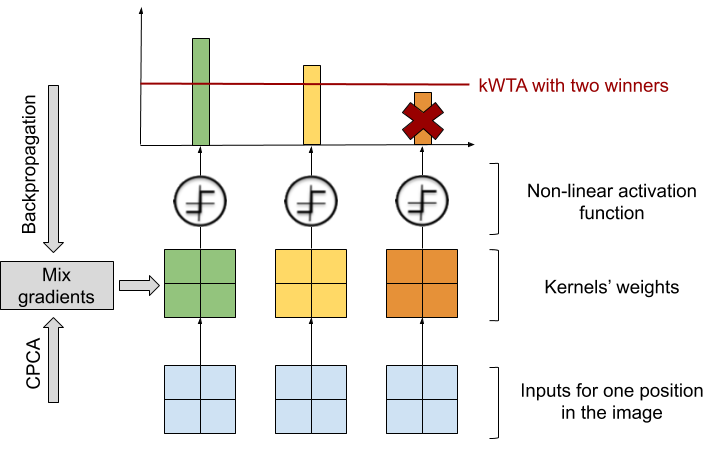
\includegraphics[width=15cm, height=10cm]{hcnn}
\caption{This figure illustrate the convolutional node of the \acrlong{hcnn}. The inputs are the same for all the kernel. The weights are used to computed the weighted sum of the inputs and the result is passed through a non-linear activation function. Then, the \acrshort{kwta} ensure that only two neurons win the competition and set the activation of the orange kernel to zero. Finally, the gradients of the backpropagation and \acrshort{cpca} are computed and mixed using the equation presented in section \ref{sec:mix_hebb_bp}.}
\label{fig:hcnn}
\end{figure}

\noindent In this model the \acrshort{kwta} competition allows to \acrshort{cpca} to learn more efficiently, i.e. conditioning function. It also brings more stability in the learning as only a subset of the neuron learn, i.e. change what they represent and react to. The \acrshort{cpca} on the other side add data-driven constraint on the way the weights are learned. This aims to avoid unrealistic pattern to be learned and can be seen as a regularization of the weights. Indeed, the equation of weights update, i.e. $\Delta w_{ij} = \epsilon y_j (x_i - w_{ij})$, shows that as the weights become large the difference between the data and weights, i.e. $x_i - w_{ij}$, become large and negative. This elegantly force the weights to remaind small.

\chapter{Model implementation} \label{model_implementation}

This chapter discuss the implementation of the \acrshort{hcnn} model. The implementation have been written from scratch and aims to provide an easily extendable framework. The code have been tested properly using unit tests and code running on the GPU have been written in order to archieve harware acceleration. The code running on the \acrshort{cpu} have been written in Java and the code executed by the \acrshort{gpu} have been written using CUDA C.

\section{Data set}

In order to make the framework easily extendable, the code provide a data set interface, which allows to load the data by batch. Support for new data sets can easily be added by creating new classes that implement this interface. As soon as a new class have been implemented, the new data set become available using the data set factory. The following line of code create an instance of the mnist data set loading the example by batch of size twenty.

$$DataSet dataSet = DataSetFactory.create("Mnist", 20);$$

\vspace{0.3cm}

\noindent The data set interface is composed of six functions:
\begin{itemize}
	\item $reload$ which retart loading the data from the begining;
	\item $hasNextBatch$ which return true if the next batch exists and false otherwise;
	\item $nextBatch$ which load the next batch;
	\item $getNumberOfClasses$ which return the number of classes to predict;
	\item $getFeatures$ which return the features of the current batch;
	\item $getLabels$ which return the labels of the current batch.
\end{itemize}

\section{Layers} \label{sec:nodes}

The code also provide a node interface, which can be used to add support for new nodes. As we will see in the next section, this generic interface allows the neural network to easily stack nodes on top of each other. The node interface is composed of three functions:
\begin{itemize}
	\item $activation$ which compute the node activation, i.e. forward pass;
	\item $update$ which update the weights, i.e. backward pass;
	\item $print$ which display the node on the standard output.
\end{itemize}

\noindent The framework currently support the following nodes:
\begin{itemize}
	\item $Dense$ which is a fully connected node;
	\item $Conv2d$ which is a 2D convolutional node supporting \acrshort{cpca} and  \acrshort{kwta};
	\item $MaxPooling2d$ which is a 2D max pooling node;
	\item $Flaten$ which transform a multi-dimensional data into a flat representation.
\end{itemize}

\noindent The following subsections focus on explaining the backpropagation of each node.

\subsection{Flaten node}

The flatten node simply reshape the data for example if the input is a 3x3 matrix the node flatten it as a vector of size 9. During the backpropagation the node will receive the derivative of the error function with respect to the each output neuron, i.e. a vector of size 9. This node does not have any weights and will just return the derivative of the error function with respect to the input, i.e. the vector of size 9 is reshape and a 3x3 matrix is returned.

\subsection{MaxPooling2d node}

The max pooling is quite similar to the flatten node, because it does not have any weights to update. During the forward pass the node keep in memory the mask that will be used to backpropagate the gradients. This mask has the same shape as the input and contains a one if the cell was the highest value of the pooling kernel and zero otherwise. Assuming a 2x2 max pooling node and a 4x4 input matrix the node will output a 2x2 matrix and keep in memory a 4x4 mask matrix. During the backward pass the node received a 2x2 matrix containing the derivative of the error function with respect to the each output neuron. The gradient are backpropagate by using the mask, indeed, each pooling kernel of the mask is multiplied by the corresponding gradient as sown in figure \ref{fig:max_pooling_bp}.

\begin{figure}[h]
\centering
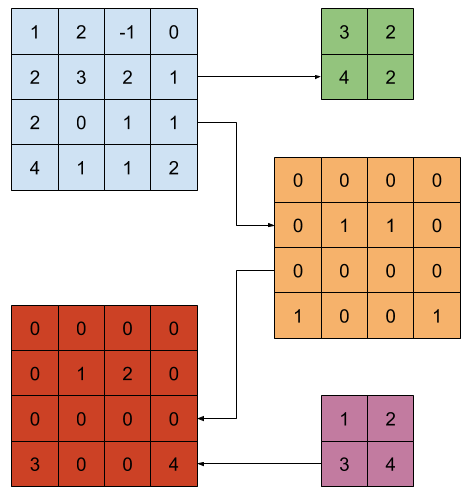
\includegraphics[width=4.5cm, height=5cm]{max_pooling_bp}
\caption{This figure illustrate the forward and backward pass of the max pooling node. The blue matrix is the input data, the green is the node output and the orange one is the mask corresponding to the input. Finally, the purple matrix is the matrix containing the derivative with respect to the output of the neurons and the red one contains the derivative with respect to the input.}
\label{fig:max_pooling_bp}
\end{figure}

\subsection{Dense node}

The dense node is more interresting, because of two reasons. First, the node has weights to update, which required to compute the derivative with respect to the weights in addition to the derivative with respect to the inputs. Second, the node has an activation function that makes the problem a bit more difficult. The first notion required to correctly explained the backpropagation in a dense node is known as the chain rule, which is defined by:

\begin{equation}
\frac{\delta z}{\delta x} = \frac{\delta z}{\delta y} \times \frac{\delta y}{\delta x}
\end{equation}

\noindent where $z$ is a function of $y$ and $y$ a function of $x$. In a dense node each neuron $j$ is computed its net input $z_j$ as a weighted sum of its inputs such as:

\begin{equation}
z_j = \sum_{i}{x_i \times w_{ij}}
\end{equation}

\noindent where $z_j$ is the net input of the j-th neuron, $x_i$ is the i-th input and $w_{ij}$ is the i-th weight of the j-th neuron. The net input is then pass through an activation function $\sigma$ such as:

\begin{equation}
y_j = \sigma(z_j)
\end{equation}

\noindent where $y_j$ is the activation of the j-th neuron. During the backpropagation the node needs to determined the derivative of the error function with respect to the weights and the inputs. The chain rules give us the following for the weights:

\begin{equation}
\frac{\delta e}{\delta w_{ij}} = \frac{\delta e}{\delta y_j} \times \frac{\delta y_j}{\delta z_j} \times \frac{\delta z_j}{\delta w_{ij}}
\end{equation}

\noindent where $\frac{\delta e}{\delta y_j}$ is the derivative of the error function with respect to the activation of the output of the j-th neuron. The derivative of the error function with respect to the input is a bit more complexe, because it required to sum over all the output neurons of the node.

\begin{equation}
\frac{\delta e}{\delta x_{i}} = \sum_{j} \frac{\delta e}{\delta y_j} \times \frac{\delta y_j}{\delta z_j} \times \frac{\delta z_j}{\delta x_i}
\end{equation}

\noindent The derivative of the error function with respect to the weights will be used to update the weights and the derivative with respect to the inputs will be used as the derivative with respect to the output of the previous node.

\subsection{Conv2d node} \label{sec:conv2d}

This section has two objectives. First, it aims to explain the backpropagation in convolutional nodes. Second, it aims to explains how to compute the \acrshort{cpca} gradients. Let's start with the computation of the backpropagation gradients for both the weights and the inputs. The only difference for the computation of the weights' gradients is the appearance of a sum over all the positions of the image where the weights have been applied:

\begin{equation} \label{eq:dwc2d}
\frac{\delta e}{\delta w_{ij}} = \sum_{k} \frac{\delta e}{\delta y_{jk}} \times \frac{\delta y_{jk}}{\delta z_{jk}} \times \frac{\delta z_{jk}}{\delta w_{ijk}}
\end{equation}

\noindent where $y_{jk}$ is the activation of the j-th neuron at the position $k$, $z_{jk}$ is the net input of the j-th neuron at the position $k$ and $w_{ijk}$ is the i-th weigth of the j-th neuron at position $k$. Note that the weights are the same for all positions $k$, but $\frac{\delta z_{jk}}{\delta w_{ijk}}$ change as $k$ change. Indeed, this derivative is actually $x_{ijk}$, i.e. the input corresponding to the $w_{ij}$ when applied at position $k$. Figure \ref{k_weights_vs_inputs} (b) aims to clarify the meaning of the position $k$. A comparable summation appear for the derivative with respect to the inputs:

\begin{equation}
\frac{\delta e}{\delta x_{i}} = \sum_{l} \sum_{j} \frac{\delta e}{\delta y_{jl}} \times \frac{\delta y_{jl}}{\delta z_{jl}} \times \frac{\delta z_{jl}}{\delta x_{il}}
\end{equation}

\noindent where $x_{il}$ is the input whose derivative is being computed; as explained the $l$ index is only relevant for the weights. Indeed, $x_{il}$ is the same input for all the value of $l$, but $\frac{\delta z_{jl}}{\delta x_{il}}$ change as $l$ change. Indeed, this derivative is actually $w_{lj}$, i.e. the weight corresponding to the input $x_{i}$ at position $l$. Figure \ref{k_weights_vs_inputs} (b) aims to clarify the meaning of the position $l$.

\begin{figure}[h]
\centering
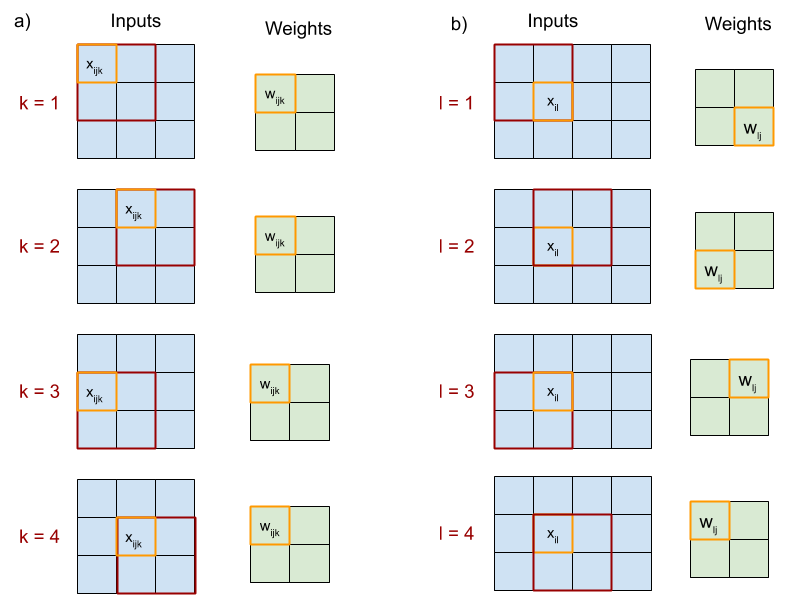
\includegraphics[width=10cm, height=8cm]{k_weights_vs_inputs}
\caption{This figure aims to clarify the meaning of the indexes $k$ and $l$. (a) The index $k$ iterate through all the positions of the input image taking steps whose size are defined by the strides of the node. (b) The index $l$ iterate through all the positions where the kernel contains the input $x_i$.}
\label{k_weights_vs_inputs}
\end{figure}

\noindent Let's now focus on the second goal of this subsection, i.e. explaining how to compute the \acrshort{cpca} gradients. The idea is to iterate through all the positions of the input image taking steps whose size are defined by the strides of the node and to compute the mean of the \acrshort{cpca} learning rule such as:

\begin{equation}
\Delta w_{ij} = \frac{\epsilon}{|K|} \sum_{k} y_{jk}(x_{ik} - w_{ij})
\end{equation}

\noindent where $w_{ij}$ is the i-th weights of the j-th neuron, $\epsilon$ is the learning rate, $|K|$ is the number of position in the image, $y_{jk}$ is the output of the neuron $j$ at position $k$ and $x_{ik}$ is the i-th input at position $k$. The constant $|K|$ can even be absorbed by the learning rate $\epsilon$ giving raise to an even simpler equation:

\begin{equation}
\Delta w_{ij} = \epsilon \sum_{k} y_{jk}(x_{ik} - w_{ij})
\end{equation}

\section{Neural Network}

The neural network class allow to build any sequential neural network, i.e. any stack of nodes. Also, it provides a $addLayer$ function that add a node on the top of stack. Its role is to wrap the stack of node and to call the $activation$ and $update$ functions when required to ensure predictions and training.

\begin{figure}[h]
\centering
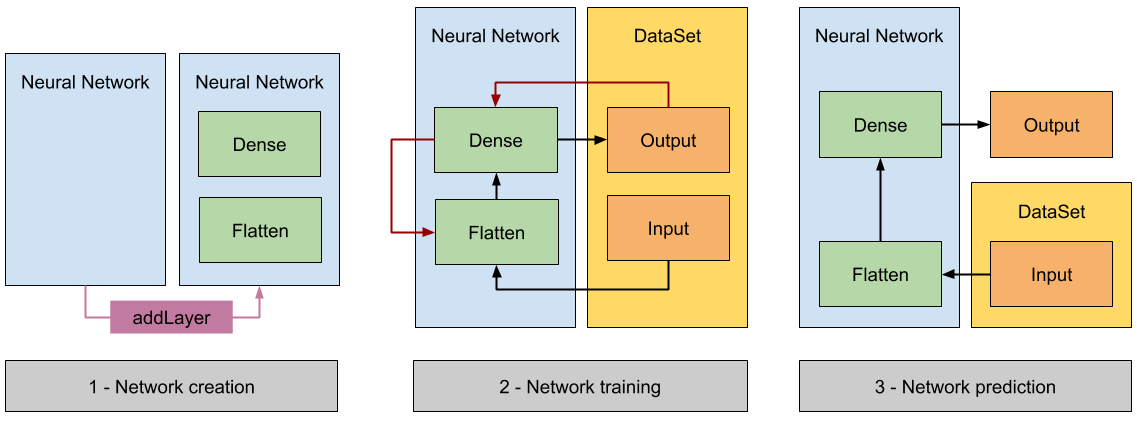
\includegraphics[width=15cm, height=5cm]{neural_network}
\caption{This figure shows how the neural network, the nodes and the data set interact with each other. The first use case shows nodes being added to the stack. The second shows the training of the network where the black arrows are calls to the $activation$ function and the red arrows the calls to the $update$ function. Finally, the third use case shows the prediction process using the same color code.}
\end{figure}

\section{Unit testing}

The unit test have been written using JUnit 5 and ensure that the code is working properly. Since, this framework is about backpropagation it is important to ensure that the gradients are correctly computed. The unit tests are implementing a technique named numerical gradient checking to check the correctness of the gradients. The key is to compute an approximation of the derivative with respect to a variable such as:
\begin{equation}
g(x) = \frac{df(x)}{dx} = \lim_{k\to0} \frac{f(x + k) - f(x - k)}{2}
\end{equation}
where $g$ is the derivative, $f$ is the function and $x$ is variable.
Figure \ref{fig:gradient_checking} illustrates the idea behind this method for the function: $f(x) = x^{2}$. A neural network can be see as a parameterized function $f$ that transform some imput $x$ into an output $f(x, \theta)$ based on the weigths $\theta$. In this context the the variable can either be $x$ or $\theta$. The approximation of the derivative is then compared with the actual value computed by the neural network.

\begin{figure}[h]
\centering
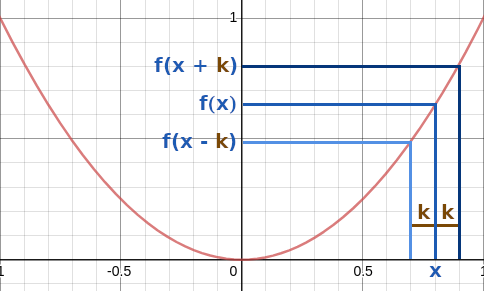
\includegraphics[width=8cm, height=5cm]{gradient_checking}
\caption{Illustration of the numerical gradient checking method.}
\label{fig:gradient_checking}
\end{figure}

\section{\acrlong{gpu}}

\subsection{Core concepts} \label{sec:core_concepts}

The \acrshort{gpu} was initially designed for graphics application where the need for parallelization is huge due to the large number of pixels to process. In order to provide such parallelization \acrshort{gpu} are generally composed of hundreds if not thousands of cores. Each core can then processes data in parallel. Originally, the API available to run code on GPU was OpenGL and DirectX, which was specialize in graphics computation. It only in November 2006 that NVIDIA unveiled the GeForce 8800 GTX built with the CUDA architechture enabling guneral-purpose computation.
\\

\begin{figure}[h]
\centering
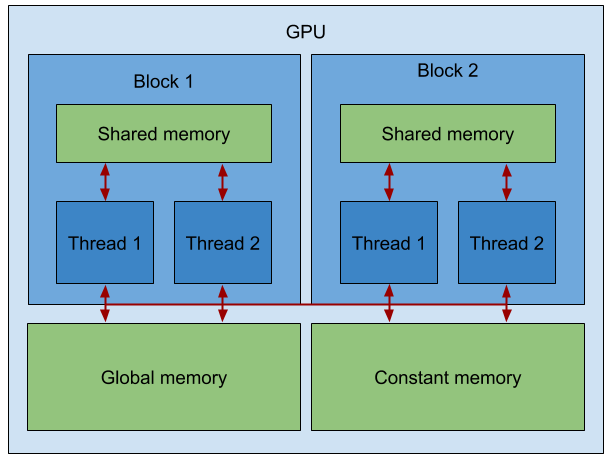
\includegraphics[width=10cm, height=6cm]{gpu_architecture}
\caption{Illustration of the GPU architecture. The red arrows link the threads to the memory they can access. The gloabal memory is the basic memory accessible from every threads. The constant memory is similar to the gloabal memory, but is accessible in read-only. Finally, the shared memory is shared amoung threads of the same block. Also, the need to syncronize the threads appears for any application that needs to reduce the shared memory, e.g. computing the sum of all the elements. This can be archieve by calling the function $\_\_syncthreads()$ to ensure that all threads finished their job.}
\label{fig:gpu_architecture}
\end{figure}

\noindent Figure \ref{fig:gpu_architecture} shows the GPU architecture. This following aims to explain how to use the CUDA API. The first thing to understand is the difference between the host and the device. The host refer to the CPU and the device refer to the GPU. A kernel is a function which run on the device and can be called from the host. A kernel does not return any value and must be annotate with the qualifier $\_\_global\_\_$, which tell the NVIDIA compiler that the function is actually a kernel.

$$\_\_global\_\_\ void\ kernel(int parameter,\ float\ *result)\ \{\ ...\ \}$$

\noindent Another important qualifier is $\_\_device\_\_$, which tell the NVIDIA compiler that the function will be executed on the device. A device function can be call from any kernel or device function.

$$\_\_device\_\_\ float\ device\_function(int\ parameter)\ \{\ ...\ \}$$

\noindent The last thing to understand is how the threads are organized. Indeed, threads are arranged into blocks and blocks are packed to form the grid. Blocks and threads can have indexes in up to three dimension. The figure \ref{fig:grid} shows a visual representation of the grid.

\begin{figure}[h]
\centering
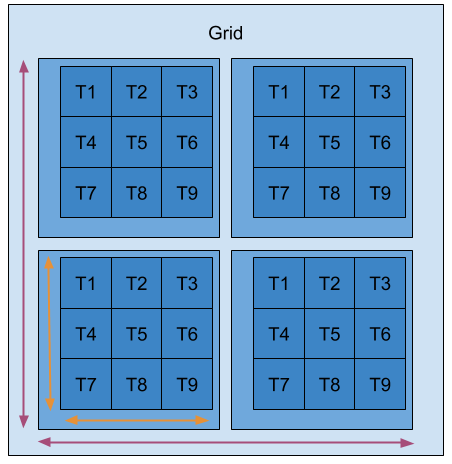
\includegraphics[width=6cm, height=5.5cm]{grid}
\caption{An example grid where both blocks and threads have 2D indexes. The purple arrows show the blocks dimensions and the orange arrows show the threads dimensions.}
\label{fig:grid}
\end{figure}

\noindent Finally, the indexes of the thread and block being processed are available in the kernel through the variables: $threadIdx.x$, $threadIdx.y$, $threadIdx.z$ and  $blockIdx.x$, $blockIdx.y$, $blockIdx.z$. Also, the number of threads and blocks are available in the kernel through the variables: $threadDim.x$, $threadDim.y$, $threadDim.z$ and  $blockDim.x$, $blockDim.y$, $blockDim.z$

\subsection{Application to neural networks}

Section \ref{sec:core_concepts} has presented all the main concepts of CUDA C, the following describes how it have been used to speed up the framework. First, it is worth noting that some computer does not have \acrshort{gpu}. Also, it is useful to provide a factory that instanciate either the \acrshort{cpu} or the \acrshort{gpu} implementation depending on the hardware available in the computer. The following line load the correct implementation for the $Conv2d$ node:

$$Conv2dInterface\ conv\_2d\ =\ TasksFactory.create("Conv2d");$$

\noindent \textcite{DBLP:journals/tjs/BritoFCSWMF16} show that \acrshort{gpu}s can be successfully used to speed up artificial neural networks. Even if the framemork has a \acrshort{gpu} implementation for all nodes presented in \ref{sec:nodes}. The following paragraphs focus on the backward pass in 2D convolutional node. Indeed, it is one of the most challenging to understand and a clear explanation will provide great insight for using \acrshort{gpu} to speed up neural networks. This kernel is using all the blocks and threads dimensions, i.e. all the following indexes are used: $threadIdx.x$, $threadIdx.y$, $threadIdx.z$, $blockIdx.x$, $blockIdx.y$ and $blockIdx.z$. The block indexes are used to go through all the weights that are stored in a 4D array, i.e. the first dimension corresponds to the number of neurons in the node, the second to the number of input channels, and finally, the third and fourth to the kernel's width and height respectively. Because there is only three blocks indexes (i.e. $x$, $y$ and $z$), the first one is used to go through the two first dimensions. As explained in section \ref{sec:conv2d} the computation of the derivatative with repect to the weights required to sum the gradients over all positions $k$, cf equation \ref{eq:dwc2d}. As previously explained, each block is responsible to compute the derivative with respect to one weight, i.e. all weights are computed in parrallel. Moreover, the threads of each block proccess several part of the images at the same time. The threads' $x$ index iterate through all the images of the batch being processed, the $y$ index trough all the vertical positions and $z$ index trough all the horizontal positions. The shared memory is used by each thread to store the sum of all the positions it is responsible. Then, the $\_\_syncthreads()$ function is called to synchronize all the threads. Finally, the first thread of each block sum the elements of the shared memory and place the result in the output buffer. The figure \ref{fig:conv2d_backpropagation} illustrate this process for a batch of two images.

\begin{figure}[h]
\centering
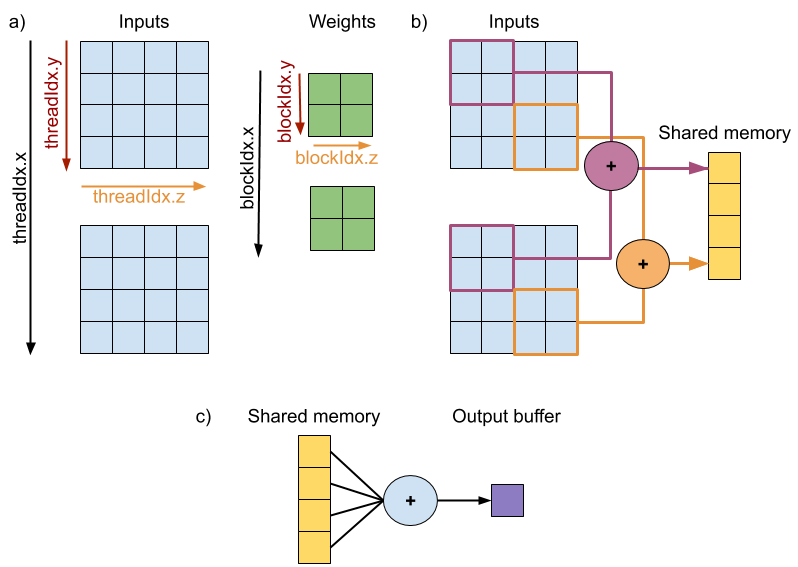
\includegraphics[width=13cm, height=10cm]{conv2d_backpropagation}
\caption{This figure illustrate the GPU-enabled backpropagation in the convolutional node. For the sake of simplicity this figure assumes two images with only one channel and two kernels of size 2x2. a) shows the meaning of the blocks and threads indexes. b) shows how the summation over all the positions is performed in parallel. This assume a 2x2 stride and a 1x2x2 grid of blocks. The first thread, i.e. purple, is responsible for the top right positions within each images. The last thread, i.e. orange, is responsible for the bottom left positions within each images. c) shows the sum of the elements in the shared memory preformed by the first thread of each block after the call to the $\_\_syncthreads()$ function.}
\label{fig:conv2d_backpropagation}
\end{figure}

\chapter{Results and Analysis} \label{result_and_analysis}

%TODO
CPU vs GPU benchmark
Learning speed
Learning robustness
Better generalization ==> less examples per class needed
Analysis of features learned

\chapter{Conclusion and Future Research} \label{conclusion}

%TODO conclude

%TODO future direction
Apply to other architechture resnet, alexnet, unet, linknet
Apply to other type of nodes dense recurrent

\printbibliography

\end{document}
